\section{包设计}
\subsection{包的设计}
本系统为了能更加有效地进行整合、生产宏观模型,就需要对系统中的类进行分组,以下是本系统中的包设计。本小结以包为单位,对每个包所含有的类及类与类间的调用关系进行说明。
\begin{figure}[!htbp]
	\centering
	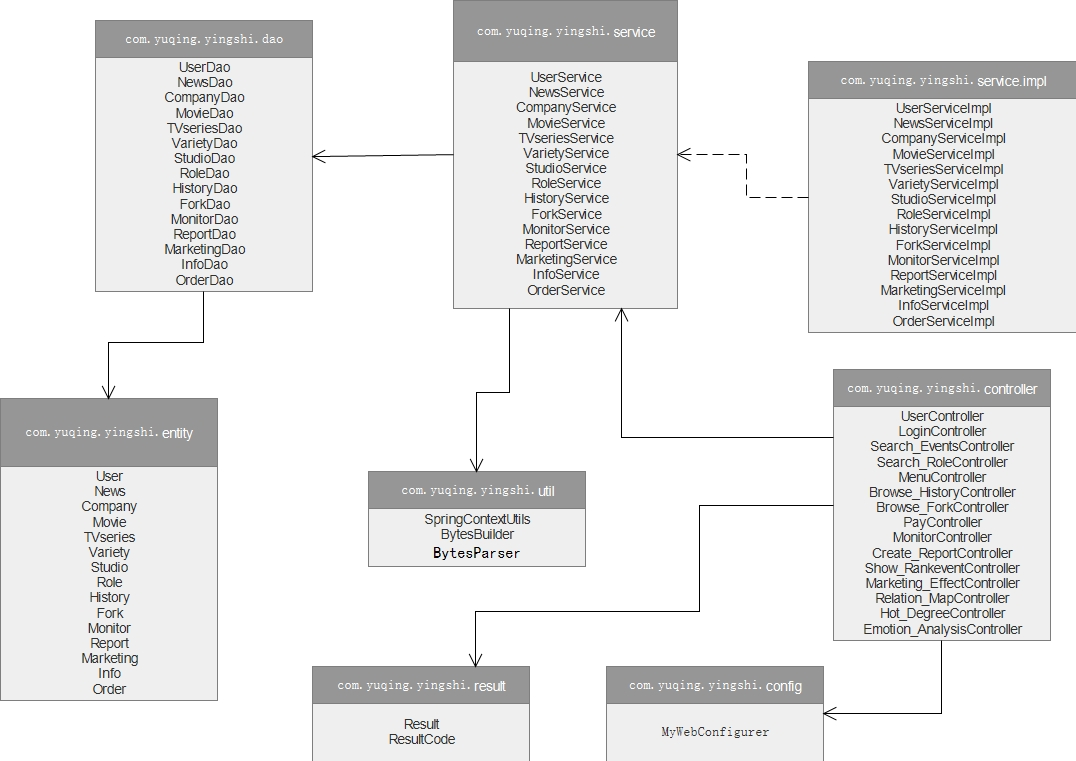
\includegraphics[scale=0.4]{image/o2.png}
	\caption{舆情系统包的设计图}
\end{figure}

下表为服务器的包设计表
\begin{tabular}{c c|} 
包名 & 
\multicolumn{2}{c}{设计说明} \\ 
\hline 
com.yuqing.yingshi.service & 该包主要存放了高层调用Dao的接口
com.yuqing.yingshi.controller & 改包主要存放了业务逻辑相关类,依赖于com.yuqing.yingshi.service,调用Service以完成业务逻辑
com.yuqing.yingshi.result& 该包存放了服务器与web端交互时返回的结果对应编码
com.yuqing.yingshi.dao&主要负责数据访问,该包中的类封装了对数据库的访问(只包含最原子的数据操作),供高层调用,依赖于com.yuqing.yingshi.entity
com.yuqing.yingshi.config& 存放了与前端web网页交互的相关配置
com.yuqing.yingshi.entity&该包主要存放数据库表中所对应的实体类
com.yuqing.yingshi.service.impl&该包存放了service包中定义的接口的具体实现
com.yuqing.yingshi.util&存放了项目相关工具类
\end{tabular}

\section{类设计}
\subsection{类的设计}

\section{接口设计}
\subsection{注册登录模块}
\subsubsection{模块内部接口}
\begin{figure}[!htbp]
	\centering
	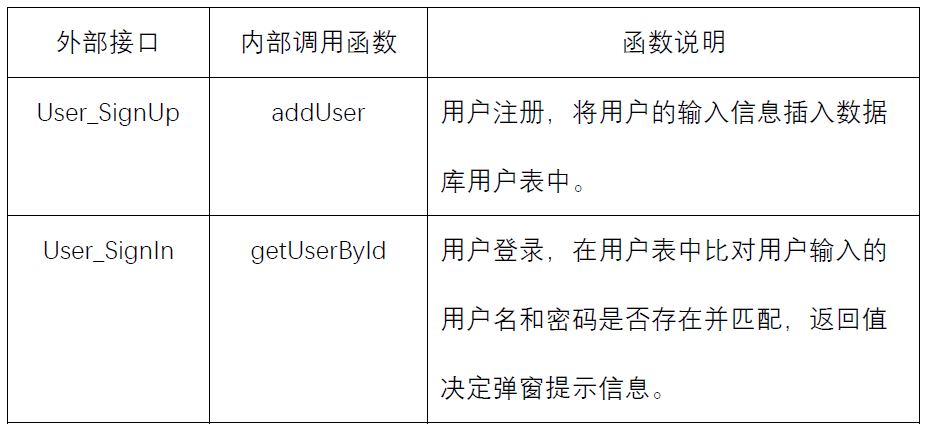
\includegraphics[scale=0.7]{image/b1.png} %修改路径下图片名称 scale 图片缩放
	\caption{注册登录模块内部接口} %修改图例(图片标题)
\end{figure}
\subsubsection{内部接口设计}
\begin{itemize}
	\item 注册实现接口
\end{itemize}
\begin{figure}[!htbp]
	\centering
	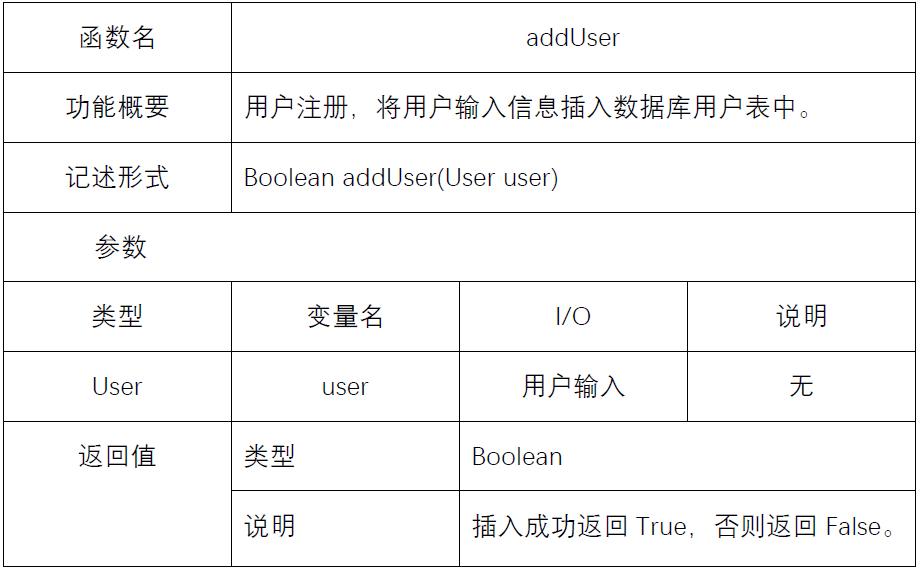
\includegraphics[scale=0.7]{image/b2.png} %修改路径下图片名称 scale 图片缩放
	\caption{注册实现接口} %修改图例(图片标题)
\end{figure}
\begin{itemize} 
	\item 登录实现接口
\end{itemize}
\begin{figure}[!htbp]
	\centering
	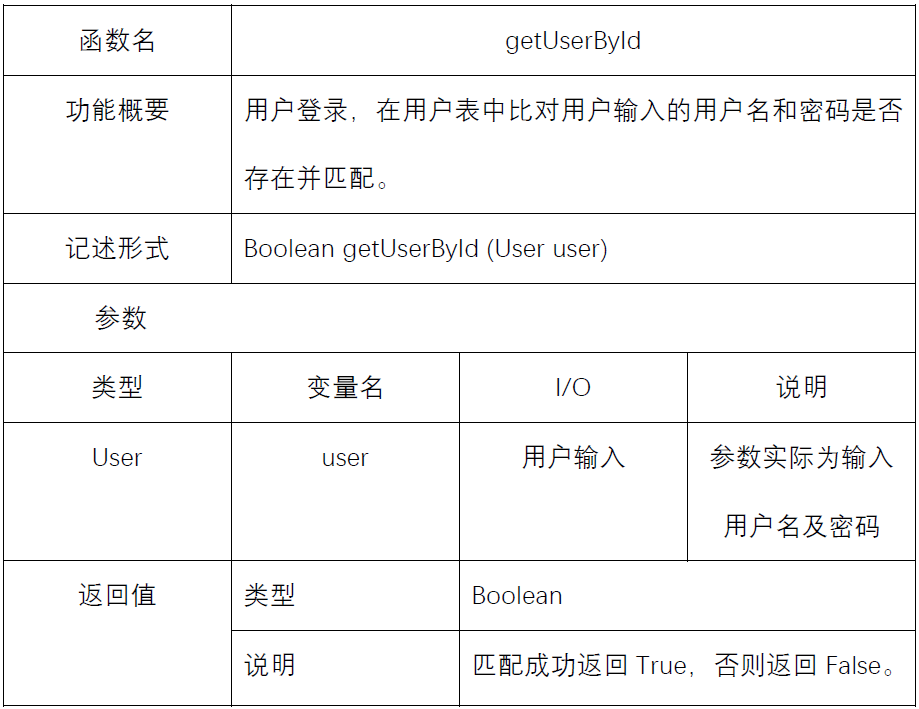
\includegraphics[scale=0.7]{image/b3.png} %修改路径下图片名称 scale 图片缩放
	\caption{登录实现接口} %修改图例(图片标题)
\end{figure}
\subsection{搜索模块}
\subsubsection{模块内部接口}
\begin{figure}[!htbp]
	\centering
	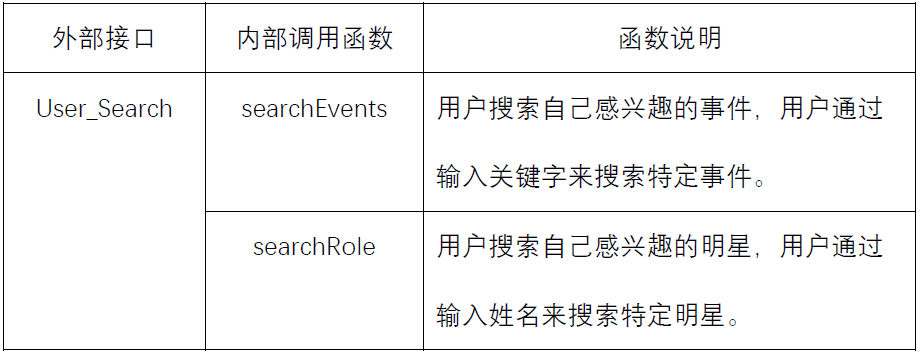
\includegraphics[scale=0.7]{image/b4.png} %修改路径下图片名称 scale 图片缩放
	\caption{搜索模块内部接口} %修改图例(图片标题)
\end{figure}
\subsubsection{内部接口设计}
\begin{itemize} 
	\item 搜索热点事件
\end{itemize}
\begin{figure}[!htbp]
	\centering
	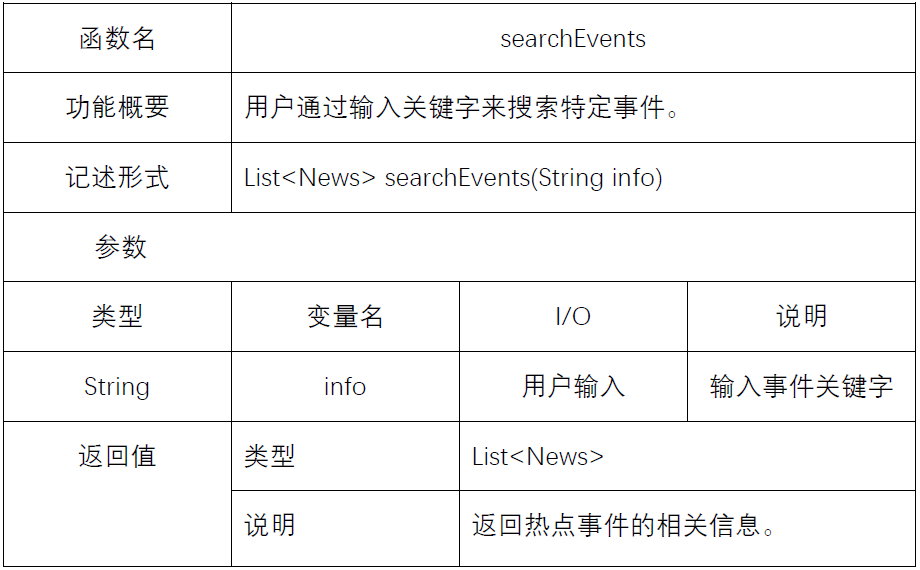
\includegraphics[scale=0.7]{image/b5.png} %修改路径下图片名称 scale 图片缩放
	\caption{搜索热点事件实现接口} %修改图例(图片标题)
\end{figure}
\begin{itemize}
	\item 搜索热点明星
\end{itemize}
\begin{figure}[!htbp]
	\centering
	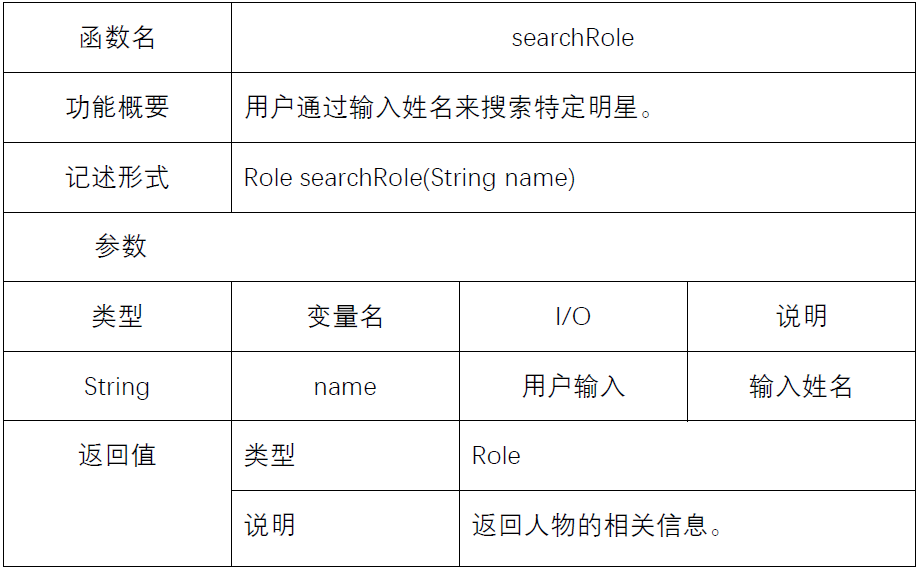
\includegraphics[scale=0.7]{image/b6.png} %修改路径下图片名称 scale 图片缩放
	\caption{搜索热点明星实现接口} %修改图例(图片标题)
\end{figure}
\subsection{展示模块}
\subsubsection{模块内部接口}
\begin{figure}[!htbp]
	\centering
	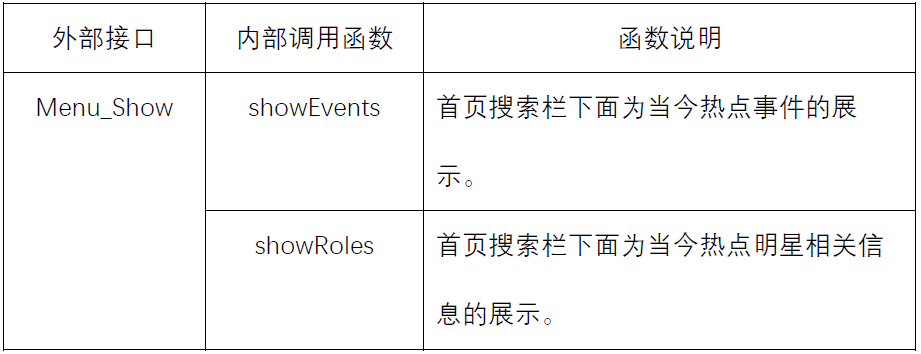
\includegraphics[scale=0.7]{image/b7.png} %修改路径下图片名称 scale 图片缩放
	\caption{展示模块内部接口} %修改图例(图片标题)
\end{figure}
\subsubsection{内部接口设计}
\begin{itemize}
	\item 展示热点事件
\end{itemize}
\begin{figure}[!htbp]
	\centering
	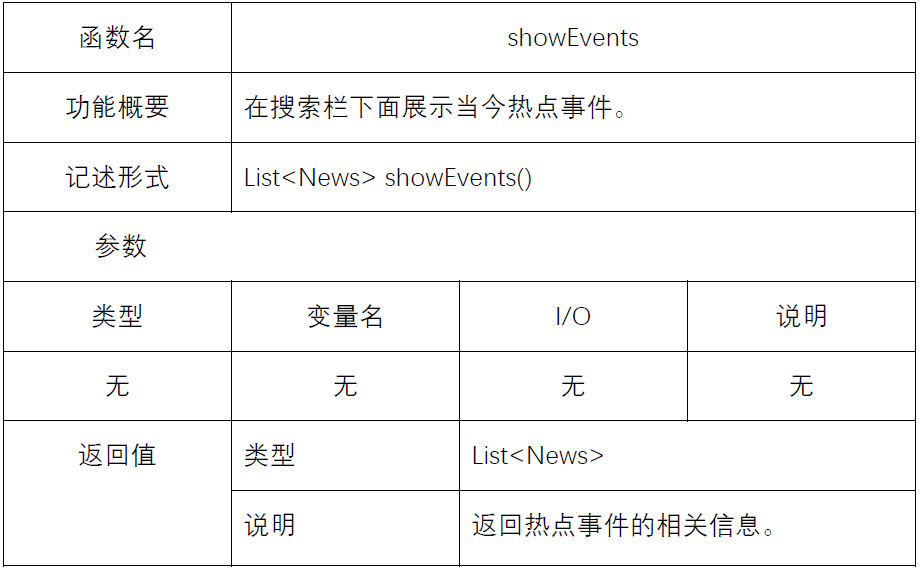
\includegraphics[scale=0.7]{image/b8.png} %修改路径下图片名称 scale 图片缩放
	\caption{展示热点事件实现接口} %修改图例(图片标题)
\end{figure}
\begin{itemize}
	\item 展示热点明星
\end{itemize}
\begin{figure}[!htbp]
	\centering
	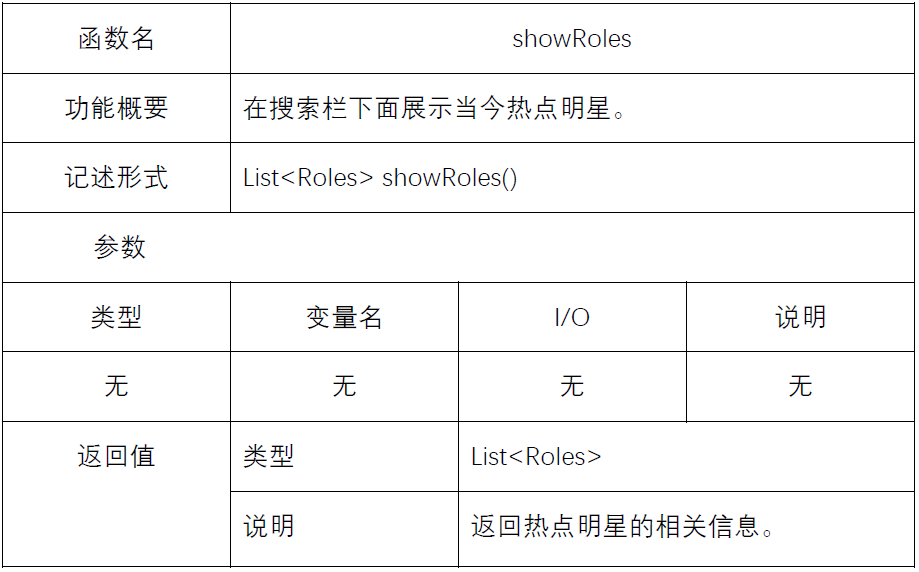
\includegraphics[scale=0.7]{image/b9.png} %修改路径下图片名称 scale 图片缩放
	\caption{展示热点明星实现接口实现} %修改图例(图片标题)
\end{figure}
\subsection{记录查询模块}
\subsubsection{模块内部接口}
\begin{figure}[!htbp]
	\centering
	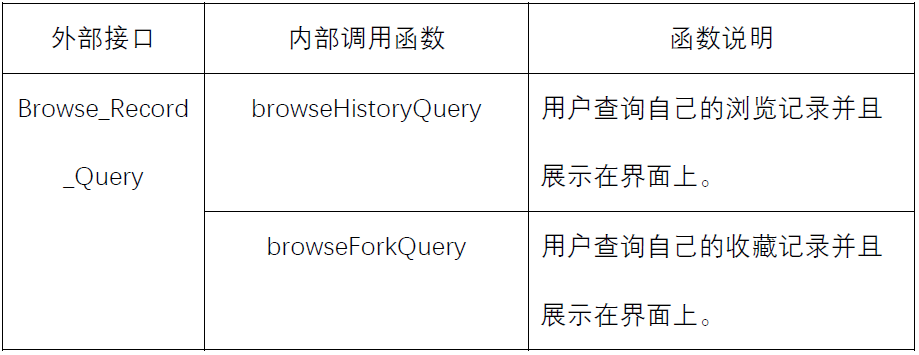
\includegraphics[scale=0.7]{image/b10.png} %修改路径下图片名称 scale 图片缩放
	\caption{记录查询模块内部接口实现} %修改图例(图片标题)
\end{figure}
\subsubsection{内部接口设计}
\begin{itemize}
	\item 查询浏览记录
\end{itemize}
\begin{figure}[!htbp]
	\centering
	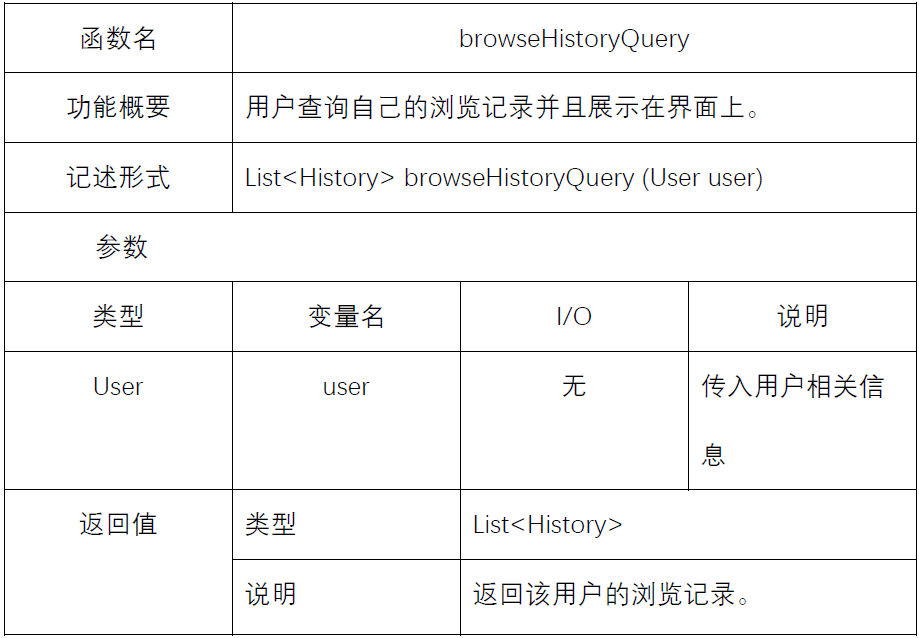
\includegraphics[scale=0.7]{image/b11.png} %修改路径下图片名称 scale 图片缩放
	\caption{查询浏览记录接口实现} %修改图例(图片标题)
\end{figure}
\begin{itemize}
	\item 查询收藏记录
\end{itemize}
\begin{figure}[!htbp]
	\centering
	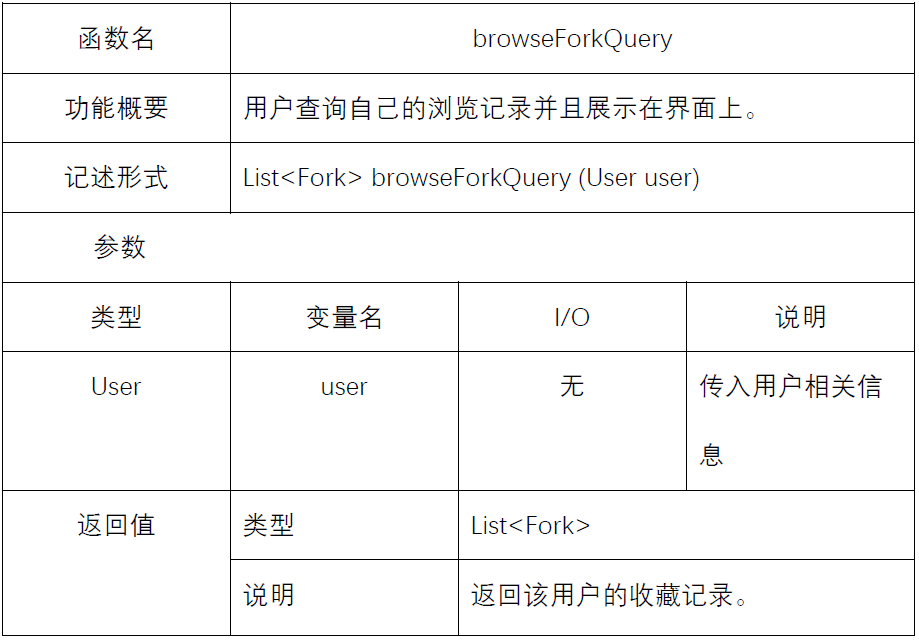
\includegraphics[scale=0.7]{image/b12.png} %修改路径下图片名称 scale 图片缩放
	\caption{查询收藏记录接口实现} %修改图例(图片标题)
\end{figure}
\subsection{支付模块}
\subsubsection{模块内部接口}
\begin{figure}[!htbp]
	\centering
	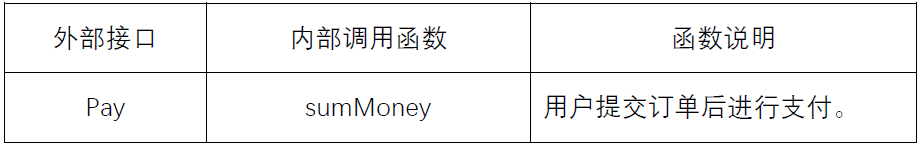
\includegraphics[scale=0.7]{image/b13.png} %修改路径下图片名称 scale 图片缩放
	\caption{支付模块内部接口} %修改图例(图片标题)
\end{figure}
\subsubsection{内部接口设计}
\begin{itemize}
	\item 支付功能
\end{itemize}
\begin{figure}[!htbp]
	\centering
	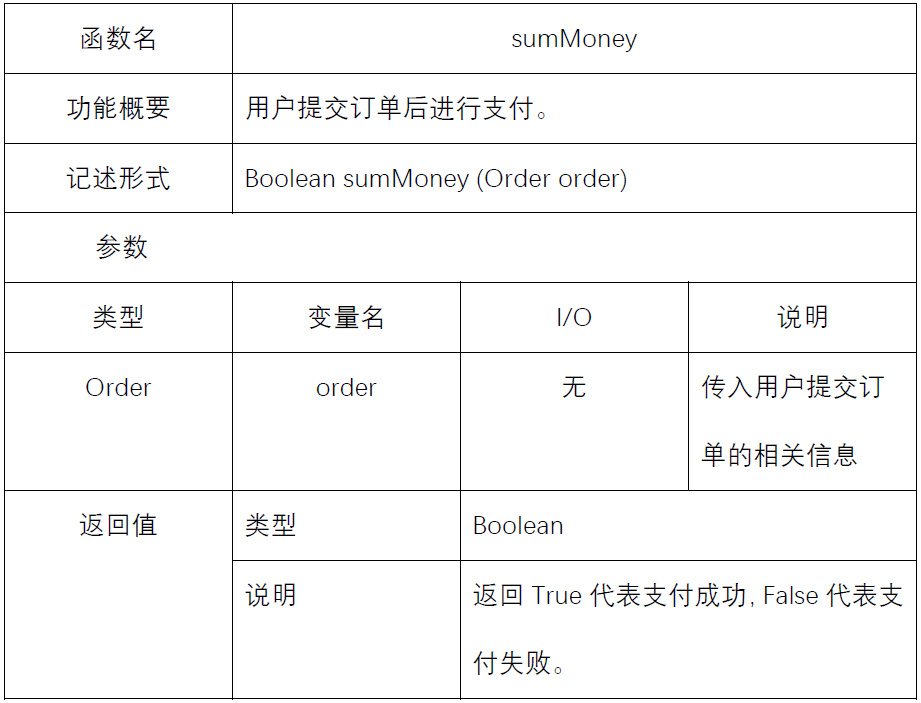
\includegraphics[scale=0.7]{image/b14.png} %修改路径下图片名称 scale 图片缩放
	\caption{支付功能接口实现} %修改图例(图片标题)
\end{figure}
\subsection{监控预警模块}
\subsubsection{模块内部接口}
\begin{figure}[!htbp]
	\centering
	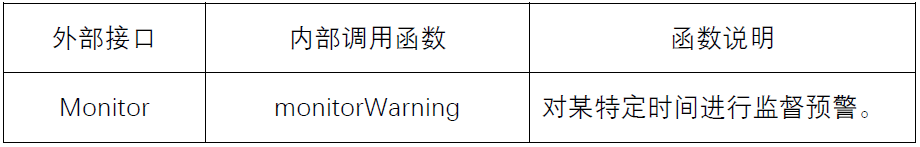
\includegraphics[scale=0.7]{image/b15.png} %修改路径下图片名称 scale 图片缩放
	\caption{监控预警模块内部接口} %修改图例(图片标题)
\end{figure}
\subsubsection{内部接口设计}
\begin{itemize}
	\item 监控预警功能
\end{itemize}
\begin{figure}[!htbp]
	\centering
	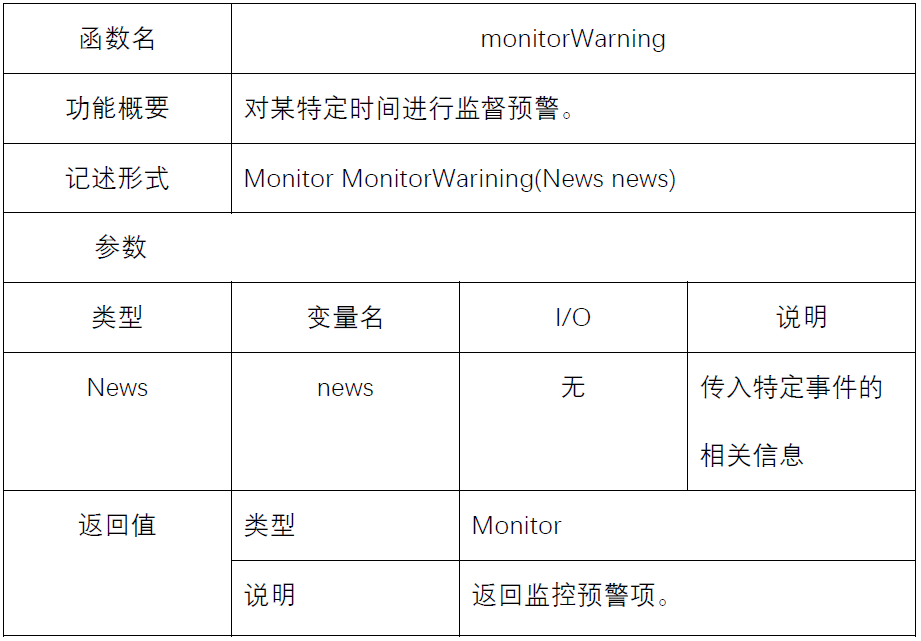
\includegraphics[scale=0.7]{image/b16.png} %修改路径下图片名称 scale 图片缩放
	\caption{监控预警功能实现} %修改图例(图片标题)
\end{figure}
\subsection{排行榜功能}
\subsubsection{模块内部接口}
\begin{figure}[!htbp]
	\centering
	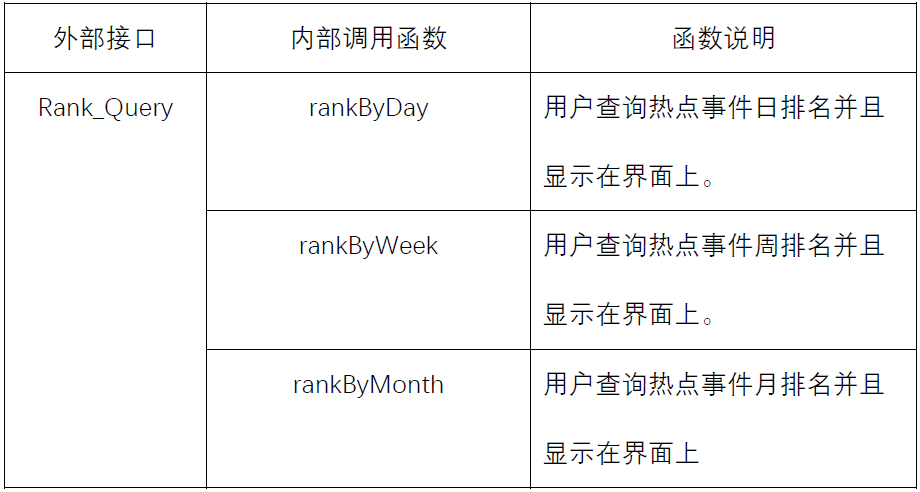
\includegraphics[scale=0.7]{image/b17.png} %修改路径下图片名称 scale 图片缩放
	\caption{排行榜模块内部接口} %修改图例(图片标题)
\end{figure}
\subsubsection{内部接口设计}
\begin{itemize}
	\item 查询日排名
\end{itemize}
\begin{figure}[!htbp]
	\centering
	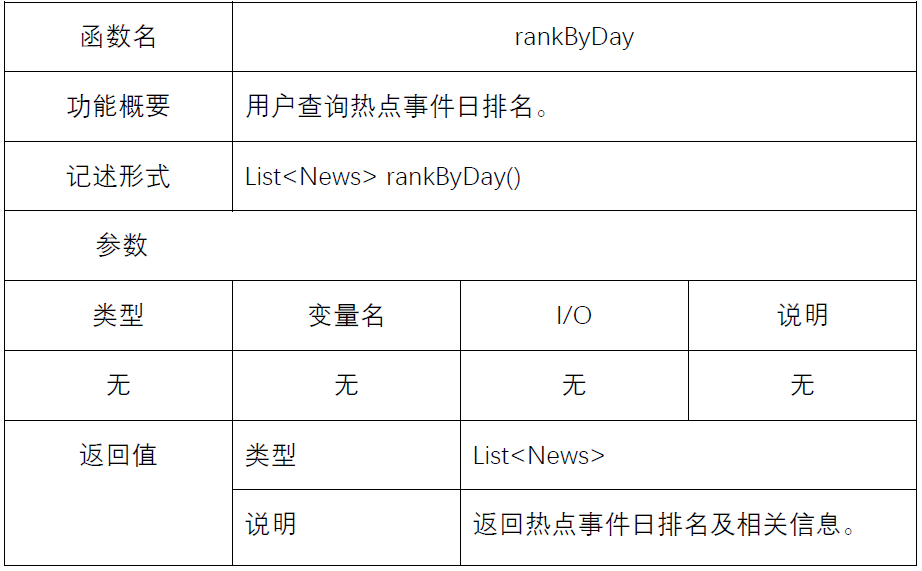
\includegraphics[scale=0.7]{image/b18.png} %修改路径下图片名称 scale 图片缩放
	\caption{查询日排名接口实现} %修改图例(图片标题)
\end{figure}
\begin{itemize}
	\item 查询周排名
\end{itemize}
\begin{figure}[!htbp]
	\centering
	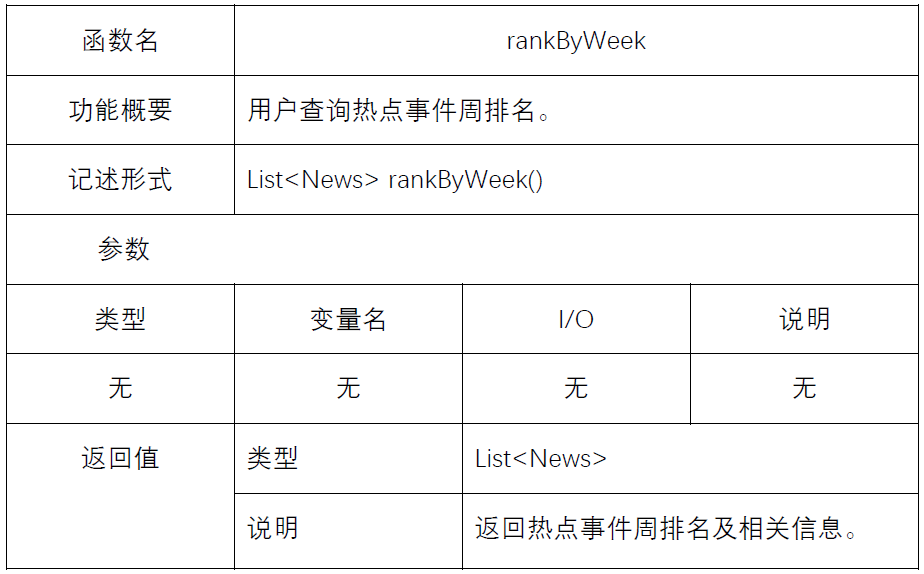
\includegraphics[scale=0.7]{image/b19.png} %修改路径下图片名称 scale 图片缩放
	\caption{查询周排名接口实现} %修改图例(图片标题)
\end{figure}
\begin{itemize}
	\item 查询月排名
\end{itemize}
\begin{figure}[!htbp]
	\centering
	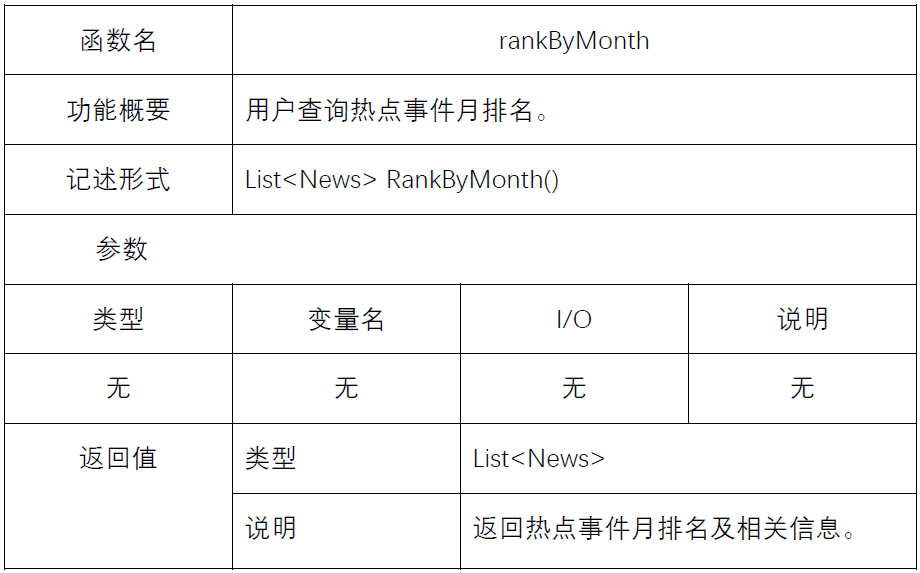
\includegraphics[scale=0.7]{image/b20.png} %修改路径下图片名称 scale 图片缩放
	\caption{查询月排名接口实现} %修改图例(图片标题)
\end{figure}
\subsection{分析模块}
\subsubsection{模块内部接口}
\begin{figure}[!htbp]
	\centering
	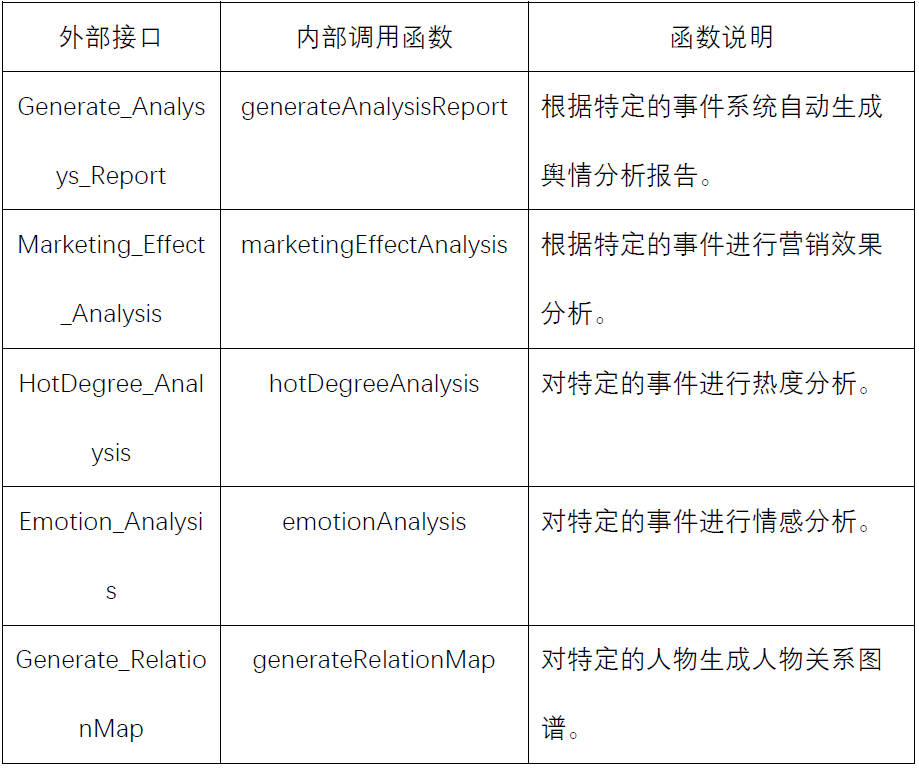
\includegraphics[scale=0.7]{image/b21.png} %修改路径下图片名称 scale 图片缩放
	\caption{分析模块内部接口} %修改图例(图片标题)
\end{figure}
\subsubsection{内部接口设计}
\begin{itemize}
	\item 生成分析报告功能
\end{itemize}
\begin{figure}[!htbp]
	\centering
	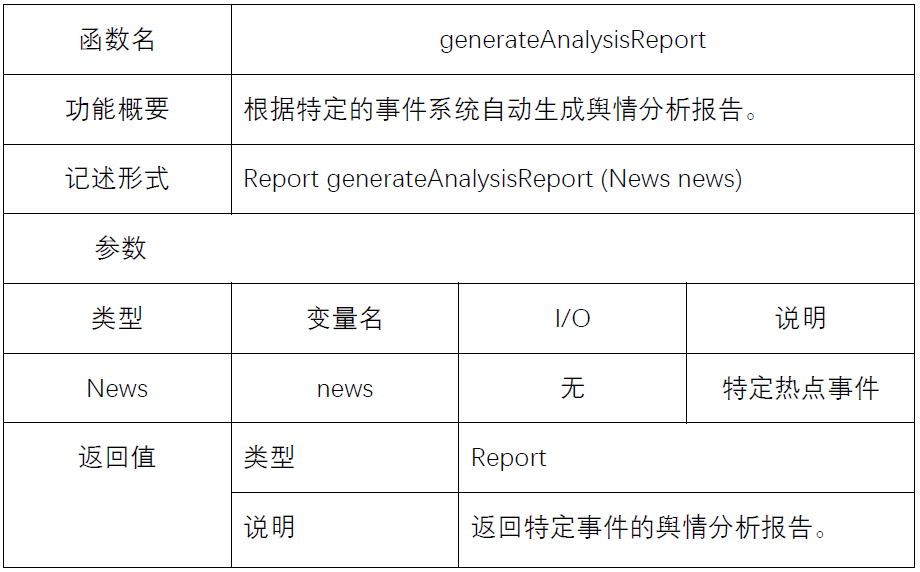
\includegraphics[scale=0.7]{image/b28.png} %修改路径下图片名称 scale 图片缩放
	\caption{生成分析报告接口实现} %修改图例(图片标题)
\end{figure}
\begin{itemize}
	\item 营销效果分析功能
\end{itemize}
\begin{figure}[!htbp]
	\centering
	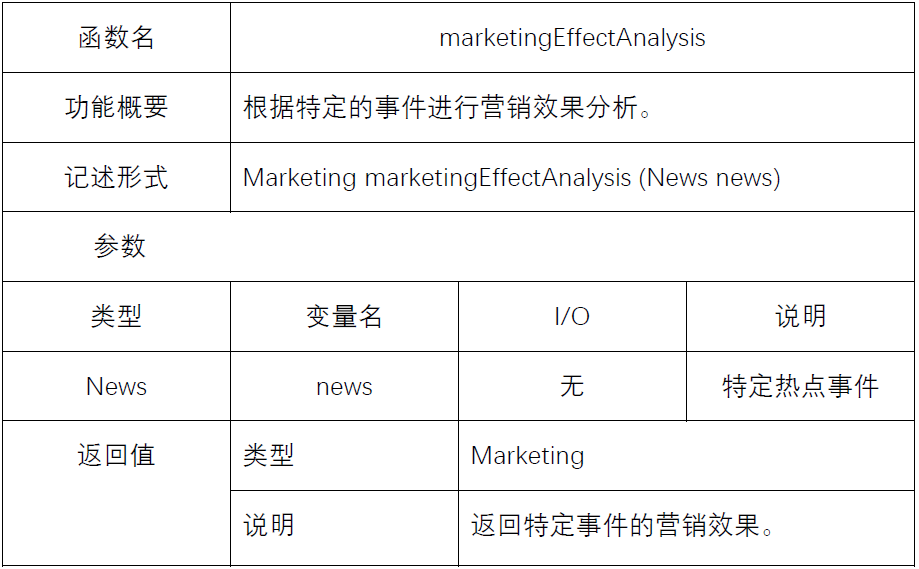
\includegraphics[scale=0.7]{image/b23.png} %修改路径下图片名称 scale 图片缩放
	\caption{营销效果分析接口实现} %修改图例(图片标题)
\end{figure}
\begin{itemize}
	\item 热度分析功能
\end{itemize}
\begin{figure}[!htbp]
	\centering
	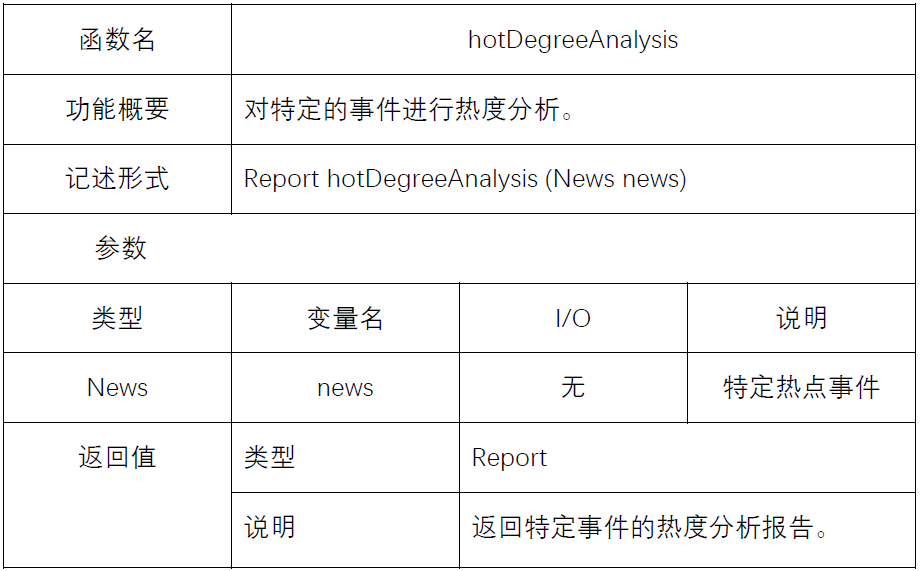
\includegraphics[scale=0.7]{image/b24.png} %修改路径下图片名称 scale 图片缩放
	\caption{热度分析接口实现} %修改图例(图片标题)
\end{figure}
\begin{itemize}
	\item 情感分析功能
\end{itemize}
\begin{figure}[!htbp]
	\centering
	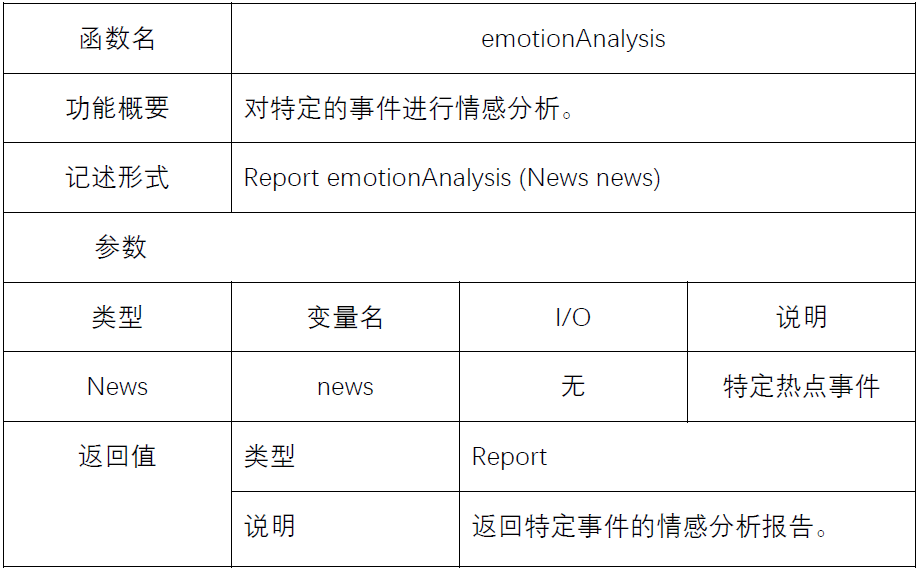
\includegraphics[scale=0.7]{image/b25.png} %修改路径下图片名称 scale 图片缩放
	\caption{情感分析接口实现} %修改图例(图片标题)
\end{figure}
\begin{itemize}
	\item 人物关系图谱功能
\end{itemize}
\begin{figure}[!htbp]
	\centering
	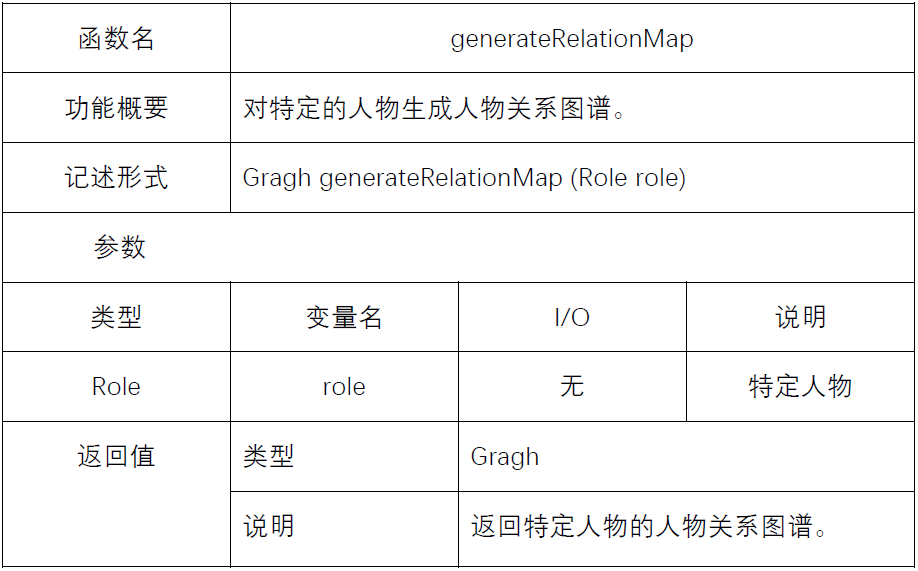
\includegraphics[scale=0.7]{image/b26.png} %修改路径下图片名称 scale 图片缩放
	\caption{生成人物关系图谱接口实现} %修改图例(图片标题)
\end{figure}
